\documentclass[11pt]{article}
\usepackage[pdftex]{graphicx}
\usepackage[finnish]{babel}
\usepackage[utf8]{inputenc}
\usepackage{amsfonts}
\usepackage{amsmath}
\usepackage{amssymb}
\usepackage{hyperref}
\usepackage{color}

\begin{document}

\title{
\Huge{\bf Joukko} \\
\Large{on shakkilauta Androidille} \\
\large{Android-ohjelmoinnin harjoitustyö}}
\author{Tuomas Starck}
\maketitle

\vspace{4em}

\section{Aiheen kuvaus}
\label{sec:aihe}

\subsection{Yleistä}

\paragraph{} Joukko on Android-alustalle kehitetty shakkipelisovellus. Joukko on pelkkä edusta (\textit{frontend}) ja vaatii toimiakseen \texttt{Sakki} pelilogiikkamoottorin, joka on saatavilla osoitteesta \url{https://github.com/hunppa/sakki}.

\paragraph{} Peli on suunniteltu kahdelle pelaajalle eikä siinä ole tekoälyvastustajaa. Joukko soveltaa nykyisiä yleisiä shakin sääntöjä sillä erotuksella, ettei sotilaan korotus upseeriksi toimi. Shakin sääntöihin voi tarvittaessa tutustua \href{http://fi.wikipedia.org/wiki/Shakki}{Wikipediasta}.

\subsection{Teknistä}

\paragraph{} Joukko käyttää OpenGL ES -rajapintaa ja Android-laitteen kiihtyvyyssensoria. Android-järjestelmät ovat tuettu versiosta 2.2 alkaen (API level 8).

\section{Käyttöliittymä}

\paragraph{} Pelin käyttöliittymä simuloi perinteistä fyysistä shakkilautaa, ja on siten hyvin pelkistetty. Käyttöliittymän peruselementti on $8\times8$~-kokoinen ruutukuvio, joka toimii pelilautana. Mikäli Android-järjestelmä sallii käyt\-tö\-liit\-ty\-män orientaation muutoksen, piirretään pelilauta aina oikein päin eli niin, että pelilaudan 1. rivi on painovoiman suunnassa.

\begin{figure}
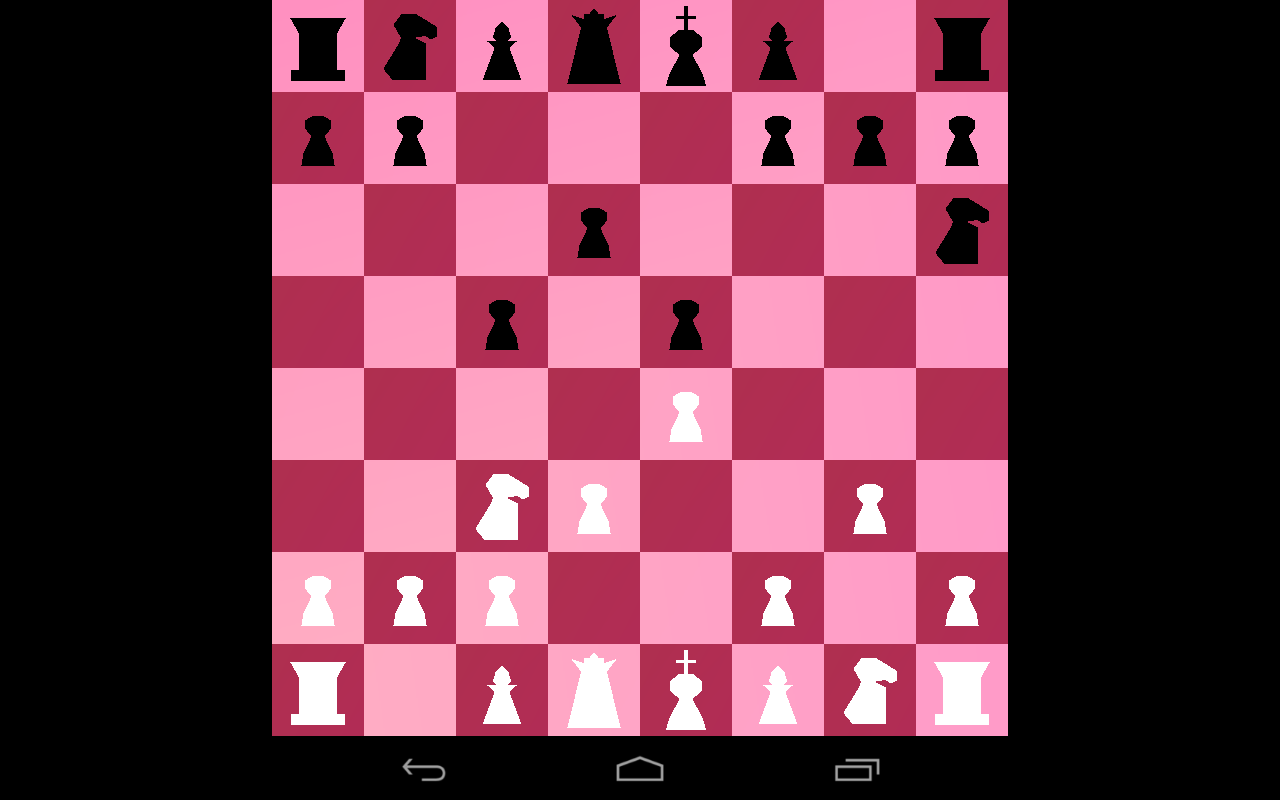
\includegraphics[width=\linewidth]{vaakakali.png}
\caption{Laite on vaakatasossa ja pelissä on valkoisen vuoro siirtää.}
\end{figure}

\paragraph{} Niin kuin shakkilaudalta voi odottaa, on sillä valkoisia ja mustia pelinappuloita. Kun pelissä on valkoisen vuoro siirtää, piirretään nappulat oikein päin suhteessa pelilaudan orientaatioon, mutta siirron jälkeen (kun on mustan pelaajan vuoro) nappulat piirretään ylösalaisin. Tämä vastaa käyttötapausta, jossa Android-laite on pelaajien välissä niin, että molemmat pelaajat ovat laitteen äärellä vastakkaisilla puolilla. Nappuloiden piirtosuunta toimii sekä visuaalisena merkkinä siitä, kumman pelaajan vuoro on että auttaa pelivuorossa olevaa pelaajaa paremmin hahmottamaan pelilaudan tilannetta.

\section{Rakenteen kuvaus}

\begin{figure}
\includegraphics[width=\linewidth]{luokkakaavio.eps}
\caption{Luokkakaavio.}
\end{figure}

\subsection{Activity}

\paragraph{} Luokka \texttt{JoukkoActivity} on sovelluksen ainoa Android \textit{Activity}. Perinteisten asioiden -- kuten Back-napin kuuntelun -- lisäksi se alustaa kiihtyvyyssensorin ja alustaa pelitilanteen tarvittaessa.

\subsection{Käyttöliittymälogiikka}

\paragraph{} Luokka \texttt{GLView} keskustelee pelilogiikan kanssa, huolehtii käyt\-tö\-liit\-ty\-mä\-lo\-gii\-kas\-ta ja ottaa vastaan käyttäjältä tulleen kosketussyötteen. \texttt{GLView}illä on apuluokka \texttt{Move}, joka ylläpitää siirron tilaa.

\subsection{Ruudunpiirto}

\paragraph{} Luokka \texttt{GLRenderer} alustaa Open GL -järjestelmän, tulkkaa kosketussyötteen käyttöliittymälle, luo piirrettävät oliot ja piirtää ne pyydettäessä.

\paragraph{} Luokat \texttt{Backdrop}, \texttt{Piecemaker} ja \texttt{Mark} ovat abstraktin luokan \texttt{Drawable} ilmentymiä ja ovat siten kaikki ruudulle piirrettäviä elementtejä. Luokat mallintavat pelilautaa, nappuloita ja visuaalista palautetta.

\paragraph{} \texttt{Figure} on staattinen luettelo, joka pitää sisällään pelinappuloiden vektorigrafiikan.

\section{Testaus}

\paragraph{} Koska Joukko on pääsääntöisesti pelkkä käyttöliittymä eikä sisällä pelilogiikkaa (ks. kappale~\ref{sec:aihe}) on siinä hyvin vähän automaattisesti testattavaa. Testaus on ollut luonteeltaan integraatiotestausta eli toteutettuja ominaisuuksia on näpytelty, hypistelty ja ravistettu kunnes ne toimivat toivotusti eivätkä mene rikki.

\section{Käyttöohje}

\subsection{Kääntäminen ja asennus}

\paragraph{} Joukko on saatavilla Eclipse-projektina osoitteesta \url{https://github.com/hunppa/joukko}. Kääntäminen vaatii, että Sakki pelilogiikkamoottori on saatavilla projektikansion alla \texttt{libs/Sakki.jar}.

\paragraph{} Sakki on saatavilla Netbeans-projektina osoitteesta \url{https://github.com/hunppa/sakki}.

\subsection{Siirto}

\paragraph{} Pelinappulan siirto tapahtuu valitsemalla ensin se ruutu, jolla nappula on ja sitten koskettamalla ruutua, jolle nappulan halutaan siirtyvän. Onnistunut valinta näkyy punaisena korostuksena. Jos siirto halutaan perua sen jälkeen, kun lähtöruudun valinta on tehty, voidaan joko koskettaa valittu ruutua uudestaan tai painaa Androidin back-painiketta.

\subsection{Shakkaus}

\paragraph{} Kun kuningas on shakattuna, piirtyy sen ruutuun keltainen merkki. Shakin sääntöjen mukaan peli voi jatkua vain, jos shakkaus puretaan. Shakkimatti-tilannetta ei erikseen tunnisteta (eikä siitä saa visuaalista tai muuta palautetta) vaan pelaajien täytyy itse ymmärtää pelin päättyneen.

\subsection{Aloitus}

\paragraph{} Pelilaudan voi palauttaa alkutilanteeseen ravistamalla Android-laitetta. \textbf{Pelin kehittäjä ei ota vastuuta ravistamalla rikotuista laitteista!}

\paragraph{Rajoitus:} Joukko ei kysy varmistusta aloitustilanteeseen palaamiseen, joten on mahdollista, että pelilaitteen varomaton käyttö saattaa pelin vahingossa alkutilaan. Tämän välttämiseksi ravistuksen täytyy olla riittävän voimakas ja terävä.

\subsection{Kumous}

\paragraph{} Androidin back-painike toimii kumous-painikkeena, jolla pääsee pelihistoriassa taaksepäin, mikäli pelihistoria on saatavilla. Kumous-toiminnolla voi myös palata edelliseen tilanteeseen silloin, kun laitetta on vahingossa ravistettu ja pelilauta on palautettu alkutilanteeseen.

\paragraph{Rajoitus:} Pelihistoriaa ei tallenneta pysyvästi, joten se tyhjentyy mm. silloin, kun laitteen orientaatio muuttuu tai Android-järjestelmä sulkee pelin.

\end{document}
